\documentclass[12pt]{article}
\usepackage[brazil]{babel}
\usepackage[utf8]{inputenc}
\usepackage[T1]{fontenc}
\usepackage{amsmath, amssymb}
\usepackage{geometry}
\usepackage{graphicx}
\usepackage{xcolor}

\definecolor{maincolor}{RGB}{0,100,50}
\usepackage{fancyhdr}
\definecolor{forestgreen}{RGB}{0,100,50}
\usepackage[most]{tcolorbox}
\newtcolorbox{block}[1]{%
  colback=green!5,
  colframe=maincolor,
  coltitle=white,
  title=#1,
  fonttitle=\bfseries,
  boxrule=1.5pt,
  arc=3mm,
  left=6pt,
  right=6pt,
  top=6pt,
  bottom=6pt
}

\geometry{margin=2.5cm}
\pagestyle{fancy}
\fancyhf{}

\renewcommand{\headrulewidth}{2pt}
\renewcommand{\footrulewidth}{2pt}

\renewcommand{\headrule}{\hbox to\headwidth{%
  \color{forestgreen}\leaders\hrule height \headrulewidth\hfill}}

\renewcommand{\footrule}{\hbox to\headwidth{%
  \color{forestgreen}\leaders\hrule height \footrulewidth\hfill}}

\setlength{\headheight}{32pt}

\fancyhead[L]{%
  
\includegraphics[height=1.2cm]{Universidade_de_Rio_Verde.jpg}
}

\fancyhead[R]{%
  \raggedleft
  \textcolor{forestgreen}{%
    \small
    \textbf{Lista de Exercícios — Programação Orientada a Objetos}\\
    Me.~Sergio Souza Novak\\
    \textit{Engenharia de Software}
  }
}

\fancyfoot[C]{%
  \textcolor{forestgreen}{\thepage}
}

\begin{document}

\vspace*{0.2cm}

\section*{Instruções}
  
   A \textbf{Programação Orientada a Objetos (POO)} é um paradigma de desenvolvimento que organiza o software a partir da modelagem de \textcolor{forestgreen}{entidades do mundo real}. Em vez de estruturar o programa apenas como uma sequência de comandos, a aplicação passa a ser composta por \textbf{objetos}, cada um possuindo \textcolor{forestgreen}{estado (atributos)} e \textcolor{forestgreen}{comportamento (métodos)}.

Durante esta unidade estudamos como transformar um \textbf{problema} em um \textcolor{forestgreen}{modelo computacional}. Para isso, aprendemos a identificar quais entidades fazem parte do sistema, quais características precisam ser armazenadas e quais ações podem ser executadas. A \textbf{classe} funciona como um molde (ou tipo abstrato), enquanto o \textbf{objeto} é a instância concreta criada a partir desse molde.

Também foi introduzido o conceito de \textbf{construtor}, responsável por inicializar corretamente o \textcolor{forestgreen}{estado inicial do objeto} no momento de sua criação, garantindo consistência dos dados. A correta utilização de \textbf{classes, atributos e métodos} é fundamental para produzir código organizado, reutilizável e de fácil manutenção --- \textcolor{forestgreen}{princípios essenciais da Engenharia de Software moderna}.

\textbf{Os exercícios desta lista têm como finalidade fixar essa etapa inicial da POO: \textcolor{forestgreen}{modelar entidades simples}, criar objetos e manipular seus estados através de métodos.}

\begin{block}{Objetivo}
Desenvolver classes em Java aplicando corretamente os conceitos de:
\begin{itemize}
    \item Classe e objeto
    \item Atributos (estado)
    \item Métodos (comportamento)
    \item Método construtor
\end{itemize}

Todos os exercícios devem conter:
\begin{itemize}
    \item Definição da classe
    \item Implementação do construtor (quando solicitado)
    \item Método \texttt{main} para instanciar objetos
\end{itemize}
\end{block}
\begin{block}{Forma de Entrega (Obrigatória)}

O aluno deverá entregar um arquivo compactado no formato \textbf{.zip}
contendo um diretório para cada exercício.

Estrutura obrigatória:
\begin{verbatim}
NomeSobrenome_Lista1.zip  
 |-- Exercicio1_Pessoa
 |    |-- Pessoa.java
 |    `-- Main.java
 |
 |-- Exercicio2_Carro
 |    |-- Carro.java
 |    `-- Main.java
 |
 |-- Exercicio3_Livro
 |    |-- Livro.java
 |    `-- Main.java
 |
 |-- Exercicio4_Aluno
 |    |-- Aluno.java
 |    `-- Main.java
 |
 |-- Exercicio5_Produto
 |    |-- Produto.java
 |    `-- Main.java
 |
 |-- Exercicio6_ContaSimples
 |    |-- ContaSimples.java
 |    `-- Main.java
 |
 |-- Exercicio7_Retangulo
 |    |-- Retangulo.java
 |    `-- Main.java
 |
 |-- Exercicio8_Funcionario
 |    |-- Funcionario.java
 |    `-- Main.java
 |
 |-- Exercicio9_Lampada
 |    |-- Lampada.java
 |    `-- Main.java
 |
 `-- Exercicio10_Termometro
      |-- Termometro.java
      `-- Main.java
\end{verbatim}


\textbf{Entrega fora do padrão estrutural implicará desconto na nota.}

\end{block}

% =======================
% EXERCÍCIOS
% =======================
\section*{Exercícios}

\begin{enumerate}

\item Crie uma classe \texttt{Pessoa} com os atributos:
\texttt{nome}, \texttt{idade} e \texttt{altura}.  
Crie dois objetos e imprima seus dados.

\begin{center}
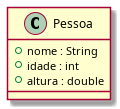
\includegraphics[width=0.3\linewidth]{pessoa.png}
\end{center}

\vspace{0.5cm}

\item Crie uma classe \texttt{Carro} com os atributos:
\texttt{marca}, \texttt{modelo}, \texttt{ano} e \texttt{velocidade}.  
Instancie dois carros com valores diferentes.

\begin{center}
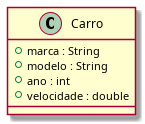
\includegraphics[width=0.3\linewidth]{carro.png}
\end{center}

\vspace{0.5cm}

\item Crie uma classe \texttt{Livro} contendo:
\texttt{titulo}, \texttt{autor}, \texttt{anoPublicacao} e \texttt{numeroPaginas}.  
Crie três objetos representando livros distintos.

\begin{center}
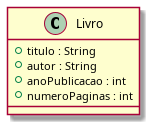
\includegraphics[width=0.3\linewidth]{livro.png}
\end{center}

\vspace{0.5cm}

\item Crie uma classe \texttt{Aluno} com:
\texttt{nome}, \texttt{matricula}, \texttt{nota1} e \texttt{nota2}.  
Implemente um construtor que receba nome e matrícula.  
Calcule e imprima a média do aluno.

\begin{center}
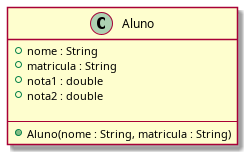
\includegraphics[width=0.5\linewidth]{aluno.png}
\end{center}

\vspace{0.5cm}

\item Crie uma classe \texttt{Produto} com:
\texttt{nome}, \texttt{preco} e \texttt{quantidade}.  
Implemente um construtor que inicialize todos os atributos.

\begin{center}
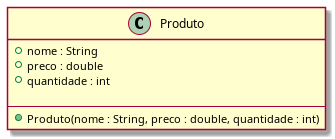
\includegraphics[width=0.7\linewidth]{produto.png}
\end{center}

\vspace{0.5cm}

\item Crie uma classe \texttt{ContaSimples} com:
\texttt{titular} e \texttt{saldo}.  
Implemente os métodos:
\begin{itemize}
    \item \texttt{depositar(double valor)}
    \item \texttt{sacar(double valor)}
    \item \texttt{exibirSaldo()}
\end{itemize}

\begin{center}
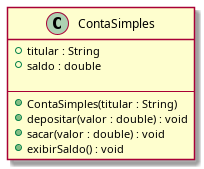
\includegraphics[width=0.6\linewidth]{contaSimples.png}
\end{center}

\vspace{0.5cm}

\item Crie uma classe \texttt{Retangulo} com:
\texttt{largura} e \texttt{altura}.  
Implemente os métodos:
\begin{itemize}
    \item \texttt{calcularArea()}
    \item \texttt{calcularPerimetro()}
\end{itemize}

\begin{center}
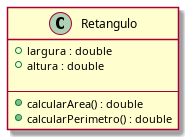
\includegraphics[width=0.3\linewidth]{retangulo.png}
\end{center}

\vspace{0.5cm}

\item Crie uma classe \texttt{Funcionario} com:
\texttt{nome} e \texttt{salario}.  
Implemente o método:
\texttt{aumentarSalario(double percentual)}.

\begin{center}
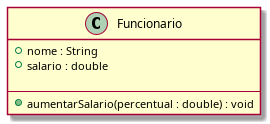
\includegraphics[width=0.5\linewidth]{funcionario.png}
\end{center}

\vspace{0.5cm}

\item Crie uma classe \texttt{Lampada} com o atributo:
\texttt{ligada} (boolean).  
Implemente os métodos:
\texttt{ligar()}, \texttt{desligar()} e \texttt{mostrarEstado()}.

\begin{center}
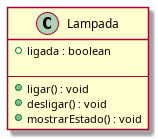
\includegraphics[width=0.3\linewidth]{lampada.png}
\end{center}

\vspace{0.5cm}

\item Crie uma classe \texttt{Termometro} com o atributo:
\texttt{temperatura}.  
Implemente métodos para aumentar, diminuir e exibir a temperatura.

\begin{center}
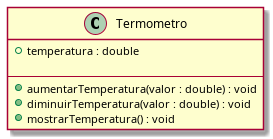
\includegraphics[width=0.5\linewidth]{termometro.png}
\end{center}

\end{enumerate}


% =======================
% GABARITO (ORIENTAÇÕES)
% =======================

\section*{Gabarito — Orientações}

\begin{block}{Estrutura Esperada}
Cada exercício deve conter:
\begin{itemize}
    \item Declaração correta da classe
    \item Declaração de atributos
    \item Implementação de construtor (quando solicitado)
    \item Implementação dos métodos
    \item Instanciação de objetos no método \texttt{main}
\end{itemize}
\end{block}

\begin{block}{Critérios de Avaliação}
\begin{itemize}
    \item Organização do código
    \item Correta manipulação do estado do objeto
    \item Uso adequado do construtor
    \item Clareza na saída exibida
\end{itemize}
\end{block}

\end{document}
